\documentclass[fleqn]{article}

\usepackage[nodisplayskipstretch]{setspace}
\usepackage{amsmath, nccmath}
\usepackage{amssymb}
\usepackage{enumitem}
\usepackage{float}
\usepackage{graphicx}

\title{Homework 1}
\author{Owen Sowatzke}
\date{September 19, 2023}

\begin{document}
	\setlength{\abovedisplayskip}{0pt}
	\setlength{\belowdisplayskip}{0pt}
	\setlength{\abovedisplayshortskip}{0pt}
	\setlength{\belowdisplayshortskip}{0pt}
	\setlength{\mathindent}{0pt}
	\doublespacing
	\maketitle
	
	\begin{enumerate}
		\item[1.] Use the graphical method to convolve the following signals. I.e., flip one signal and slide it across the other signal. Show graphs to illustrate your steps.
		
		$h[n] = 0.5\delta[n] - 0.25\delta[n-1]$
		
		$x[n] = (n+1)u[n]u[2-n]$
		
		The convolution output $y[n]$ is given by the following formula:
		
		\begin{align*}
			y[n] = \sum_{k=-\infty}^{\infty}{x[k]h[n-k]}
		\end{align*}
		
		To graphically convolve the signals, we need to form plots of $x[k]$ and \newline $h[n-k]$. The output $y[n]$ can be generated for each value of $n$ by multiplying $x[k]$ with $h[n-k]$ and summing the result.
		
		Start by plotting $x[n]$ and $h[n]$ as illustrated in Figure \ref{prob1_xn_plot} and in Figure \ref{prob1_hn_plot} respectively.
		
		\begin{figure}[H]				
			\centerline{\fbox{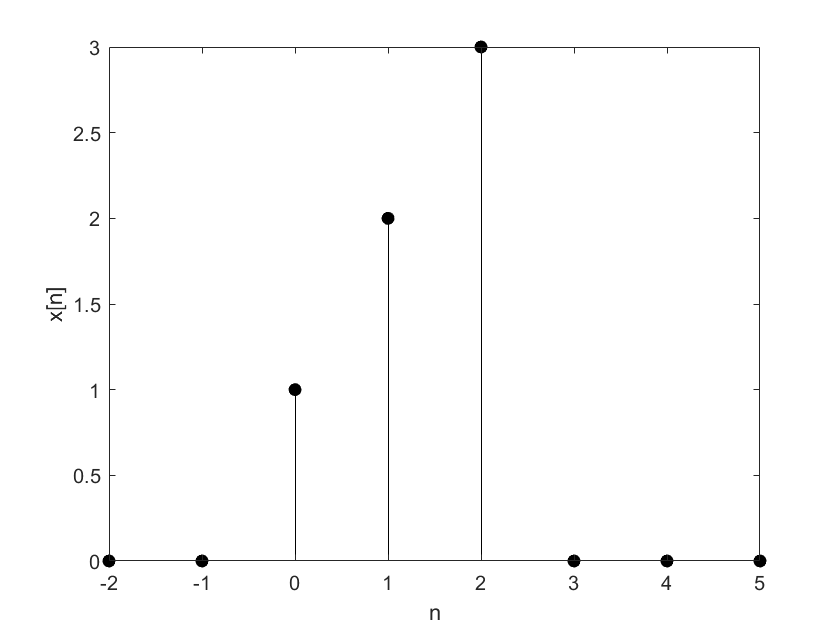
\includegraphics[width=0.5\textwidth]{prob1_xn_plot.png}}}
			\caption{Plot of $x[n]$}
			\label{prob1_xn_plot}
		\end{figure}
		
		\begin{figure}[H]				
			\centerline{\fbox{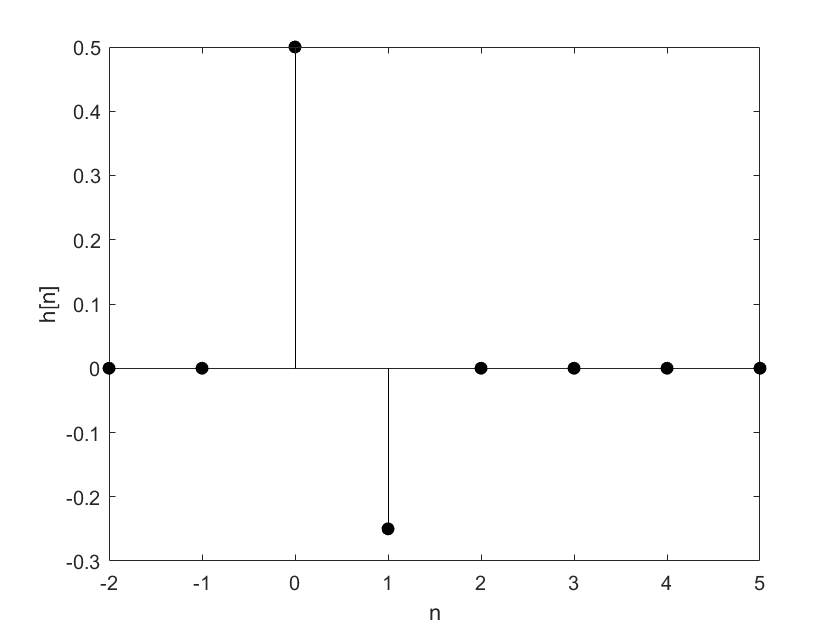
\includegraphics[width=0.5\textwidth]{prob1_hn_plot.png}}}
			\caption{Plot of $h[n]$}
			\label{prob1_hn_plot}
		\end{figure}
		
		Next, plot $x[k]$ and $h[k]$ as illustrated in Figure \ref{prob1_xk_plot} and Figure \ref{prob1_hk_plot} respectively. 
		
		\begin{figure}[H]				
			\centerline{\fbox{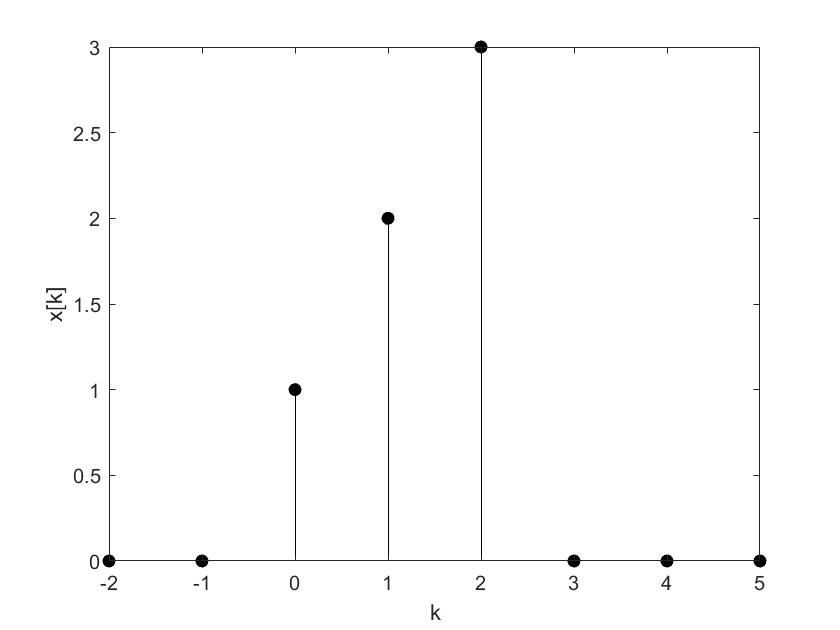
\includegraphics[width=0.5\textwidth]{prob1_xk_plot.png}}}
			\caption{Plot of $x[k]$}
			\label{prob1_xk_plot}
		\end{figure}
		
		\begin{figure}[H]				
			\centerline{\fbox{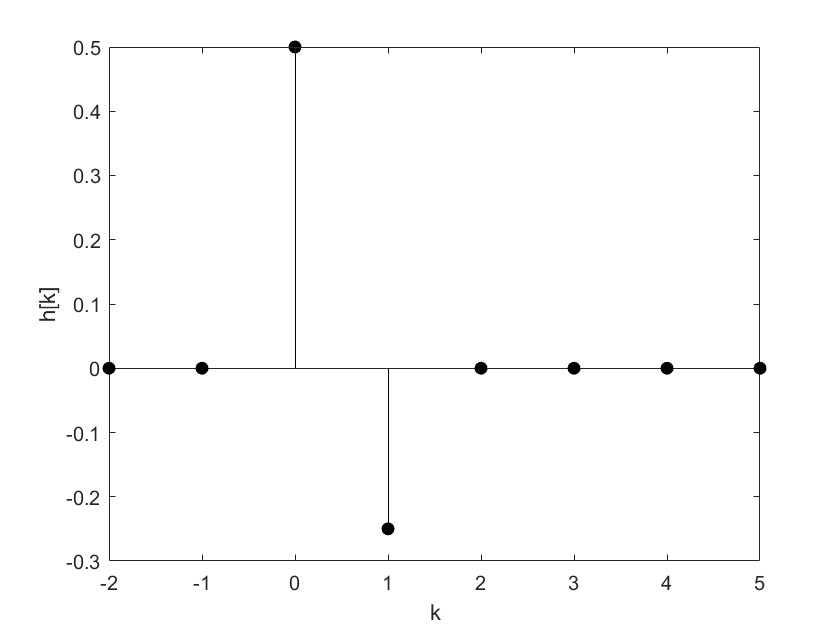
\includegraphics[width=0.5\textwidth]{prob1_hk_plot.png}}}
			\caption{Plot of $h[k]$}
			\label{prob1_hk_plot}
		\end{figure}
		
		Then, flip $h[k]$ to obtain $h[-k]$ and plot the result as shown in Figure \ref{prob1_h-k_plot}.
		
		\begin{figure}[H]				
			\centerline{\fbox{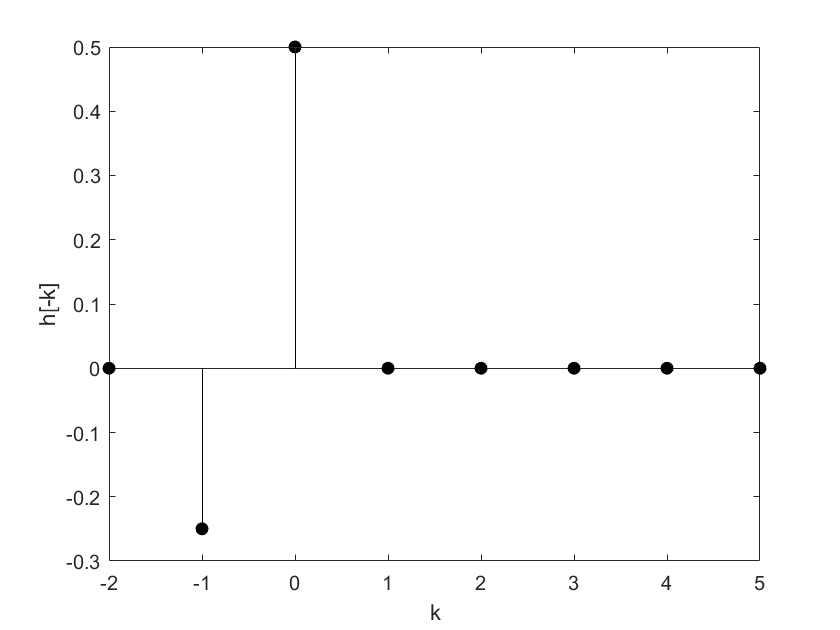
\includegraphics[width=0.5\textwidth]{prob1_h-k_plot.png}}}
			\caption{Plot of $h[-k]$}
			\label{prob1_h-k_plot}
		\end{figure}
		
		Now, shift $h[-k]$ by $n$ to obtain $h[n-k]$ and plot the result as shown in Figure \ref{prob1_hn-k_plot}.
		
		\begin{figure}[H]				
			\centerline{\fbox{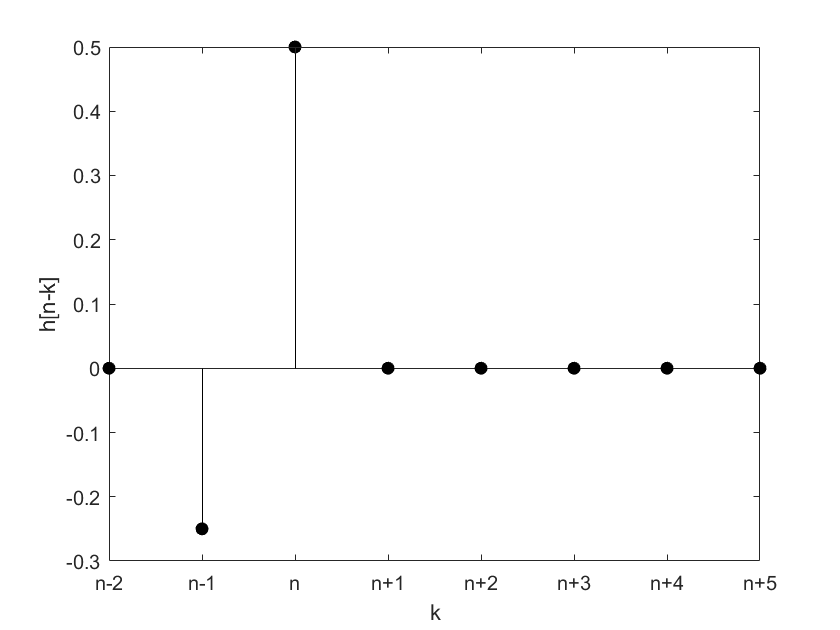
\includegraphics[width=0.5\textwidth]{prob1_hn-k_plot.png}}}
			\caption{Plot of $h[n-k]$}
			\label{prob1_hn-k_plot}
		\end{figure}
		
		For each value of $n$, multiply $x[k]$ by $h[n-k]$ and sum the result.
		
		For $n < 0$:
		
		$y[n] = 0$
		
		$y[0] = 0.5(1) = 0.5$
		
		$y[1] = 0.5(2) - 0.25(1) = 1 - 0.25 = 0.75$
		
		$y[2] = 0.5(3) - 0.25(2) = 1.5 - 0.5 = 1$
		
		$y[3] = -0.25(3) = -0.75$
		
		For $n > 3$:
		
		$y[n] = 0$:
		
		$\mathbf{\therefore y[n] = 0.5\delta[n] + 0.75\delta[n-1] + \delta[n-2] - 0.75\delta[n-3]}$
		
		The result $y[n]$ is plotted in Figure \ref{prob1_yn_plot}.
		
		\begin{figure}[H]				
			\centerline{\fbox{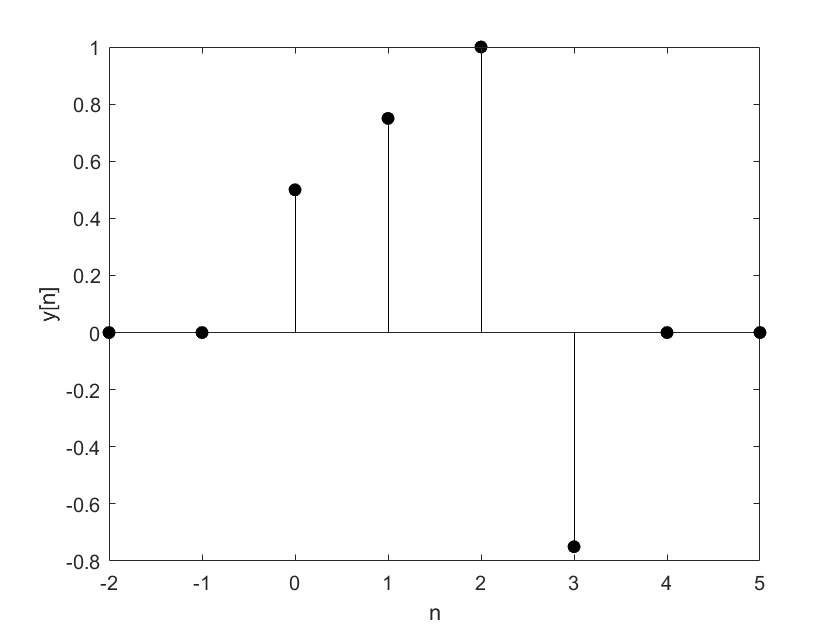
\includegraphics[width=0.5\textwidth]{prob1_yn_plot.png}}}
			\caption{Plot of $y[n]$}
			\label{prob1_yn_plot}
		\end{figure}
		
		\item[2.] Evaluate the convolution sum mathematically (i.e., do not use the graphical method) to obtain the unit step response of an LTI system whose impulse response is
		
		$h[n] = 3^{-n}u[n]$
		
		\begin{align*}
			y[n] = \sum_{k = -\infty}^{\infty}{x[k]h[n-k]} = \sum_{k = -\infty}^{\infty}{h[k]x[n-k]} = \sum_{k = -\infty}^{\infty}{3^{-k}u[k]u[n-k]}
		\end{align*}
		
		\begin{align*}
			= \sum_{k = 0}^{\infty}{3^{-k}u[n-k]}
		\end{align*}
		
		For $n < 0$:
		
		$y[n] = 0$
		
		For $n \geq 0$:
		
		\begin{align*}
			y[n] = \sum_{k = 0}^{n}{3^{-k}} = \sum_{k = 0}^{n}{(3^{-1})^k} = \sum_{k = 0}^{n}{\left(\frac{1}{3}\right)^k} = \frac{1-\left(\frac{1}{3}\right)^{n+1}}{1-\frac{1}{3}}
		\end{align*}
		
		\begin{align*}
			 = \frac{3\left(1-\left(\frac{1}{3}\right)^{n+1}\right)}{3\left(1-\frac{1}{3}\right)} = \frac{3-3\left(\frac{1}{3}\right)^{n+1}}{3-1} = \frac{3-\left(\frac{1}{3}\right)^{n}}{2} = \frac{1}{2}\left(3-\left(\frac{1}{3}\right)^{n}\right)
		\end{align*}
		
		\begin{align*}
			\mathbf{\therefore y[n] = \frac{1}{2}\left(3-\left(\frac{1}{3}\right)^{n}\right)u[n]}
		\end{align*}
	\end{enumerate}
	
\end{document}